% Options for packages loaded elsewhere
\PassOptionsToPackage{unicode}{hyperref}
\PassOptionsToPackage{hyphens}{url}
%
\documentclass[
]{article}
\usepackage{lmodern}
\usepackage{amssymb,amsmath}
\usepackage{ifxetex,ifluatex}
\ifnum 0\ifxetex 1\fi\ifluatex 1\fi=0 % if pdftex
  \usepackage[T1]{fontenc}
  \usepackage[utf8]{inputenc}
  \usepackage{textcomp} % provide euro and other symbols
\else % if luatex or xetex
  \usepackage{unicode-math}
  \defaultfontfeatures{Scale=MatchLowercase}
  \defaultfontfeatures[\rmfamily]{Ligatures=TeX,Scale=1}
\fi
% Use upquote if available, for straight quotes in verbatim environments
\IfFileExists{upquote.sty}{\usepackage{upquote}}{}
\IfFileExists{microtype.sty}{% use microtype if available
  \usepackage[]{microtype}
  \UseMicrotypeSet[protrusion]{basicmath} % disable protrusion for tt fonts
}{}
\makeatletter
\@ifundefined{KOMAClassName}{% if non-KOMA class
  \IfFileExists{parskip.sty}{%
    \usepackage{parskip}
  }{% else
    \setlength{\parindent}{0pt}
    \setlength{\parskip}{6pt plus 2pt minus 1pt}}
}{% if KOMA class
  \KOMAoptions{parskip=half}}
\makeatother
\usepackage{xcolor}
\IfFileExists{xurl.sty}{\usepackage{xurl}}{} % add URL line breaks if available
\IfFileExists{bookmark.sty}{\usepackage{bookmark}}{\usepackage{hyperref}}
\hypersetup{
  pdftitle={Flujo de análisis en clasificación supervisada},
  pdfauthor={Laura Rodríguez Navas},
  hidelinks,
  pdfcreator={LaTeX via pandoc}}
\urlstyle{same} % disable monospaced font for URLs
\usepackage[margin=1in]{geometry}
\usepackage{color}
\usepackage{fancyvrb}
\newcommand{\VerbBar}{|}
\newcommand{\VERB}{\Verb[commandchars=\\\{\}]}
\DefineVerbatimEnvironment{Highlighting}{Verbatim}{commandchars=\\\{\}}
% Add ',fontsize=\small' for more characters per line
\usepackage{framed}
\definecolor{shadecolor}{RGB}{248,248,248}
\newenvironment{Shaded}{\begin{snugshade}}{\end{snugshade}}
\newcommand{\AlertTok}[1]{\textcolor[rgb]{0.94,0.16,0.16}{#1}}
\newcommand{\AnnotationTok}[1]{\textcolor[rgb]{0.56,0.35,0.01}{\textbf{\textit{#1}}}}
\newcommand{\AttributeTok}[1]{\textcolor[rgb]{0.77,0.63,0.00}{#1}}
\newcommand{\BaseNTok}[1]{\textcolor[rgb]{0.00,0.00,0.81}{#1}}
\newcommand{\BuiltInTok}[1]{#1}
\newcommand{\CharTok}[1]{\textcolor[rgb]{0.31,0.60,0.02}{#1}}
\newcommand{\CommentTok}[1]{\textcolor[rgb]{0.56,0.35,0.01}{\textit{#1}}}
\newcommand{\CommentVarTok}[1]{\textcolor[rgb]{0.56,0.35,0.01}{\textbf{\textit{#1}}}}
\newcommand{\ConstantTok}[1]{\textcolor[rgb]{0.00,0.00,0.00}{#1}}
\newcommand{\ControlFlowTok}[1]{\textcolor[rgb]{0.13,0.29,0.53}{\textbf{#1}}}
\newcommand{\DataTypeTok}[1]{\textcolor[rgb]{0.13,0.29,0.53}{#1}}
\newcommand{\DecValTok}[1]{\textcolor[rgb]{0.00,0.00,0.81}{#1}}
\newcommand{\DocumentationTok}[1]{\textcolor[rgb]{0.56,0.35,0.01}{\textbf{\textit{#1}}}}
\newcommand{\ErrorTok}[1]{\textcolor[rgb]{0.64,0.00,0.00}{\textbf{#1}}}
\newcommand{\ExtensionTok}[1]{#1}
\newcommand{\FloatTok}[1]{\textcolor[rgb]{0.00,0.00,0.81}{#1}}
\newcommand{\FunctionTok}[1]{\textcolor[rgb]{0.00,0.00,0.00}{#1}}
\newcommand{\ImportTok}[1]{#1}
\newcommand{\InformationTok}[1]{\textcolor[rgb]{0.56,0.35,0.01}{\textbf{\textit{#1}}}}
\newcommand{\KeywordTok}[1]{\textcolor[rgb]{0.13,0.29,0.53}{\textbf{#1}}}
\newcommand{\NormalTok}[1]{#1}
\newcommand{\OperatorTok}[1]{\textcolor[rgb]{0.81,0.36,0.00}{\textbf{#1}}}
\newcommand{\OtherTok}[1]{\textcolor[rgb]{0.56,0.35,0.01}{#1}}
\newcommand{\PreprocessorTok}[1]{\textcolor[rgb]{0.56,0.35,0.01}{\textit{#1}}}
\newcommand{\RegionMarkerTok}[1]{#1}
\newcommand{\SpecialCharTok}[1]{\textcolor[rgb]{0.00,0.00,0.00}{#1}}
\newcommand{\SpecialStringTok}[1]{\textcolor[rgb]{0.31,0.60,0.02}{#1}}
\newcommand{\StringTok}[1]{\textcolor[rgb]{0.31,0.60,0.02}{#1}}
\newcommand{\VariableTok}[1]{\textcolor[rgb]{0.00,0.00,0.00}{#1}}
\newcommand{\VerbatimStringTok}[1]{\textcolor[rgb]{0.31,0.60,0.02}{#1}}
\newcommand{\WarningTok}[1]{\textcolor[rgb]{0.56,0.35,0.01}{\textbf{\textit{#1}}}}
\usepackage{graphicx,grffile}
\makeatletter
\def\maxwidth{\ifdim\Gin@nat@width>\linewidth\linewidth\else\Gin@nat@width\fi}
\def\maxheight{\ifdim\Gin@nat@height>\textheight\textheight\else\Gin@nat@height\fi}
\makeatother
% Scale images if necessary, so that they will not overflow the page
% margins by default, and it is still possible to overwrite the defaults
% using explicit options in \includegraphics[width, height, ...]{}
\setkeys{Gin}{width=\maxwidth,height=\maxheight,keepaspectratio}
% Set default figure placement to htbp
\makeatletter
\def\fps@figure{htbp}
\makeatother
\setlength{\emergencystretch}{3em} % prevent overfull lines
\providecommand{\tightlist}{%
  \setlength{\itemsep}{0pt}\setlength{\parskip}{0pt}}
\setcounter{secnumdepth}{-\maxdimen} % remove section numbering

\title{Flujo de análisis en clasificación supervisada}
\usepackage{etoolbox}
\makeatletter
\providecommand{\subtitle}[1]{% add subtitle to \maketitle
  \apptocmd{\@title}{\par {\large #1 \par}}{}{}
}
\makeatother
\subtitle{Métodos supervisados}
\author{Laura Rodríguez Navas}
\date{Septiembre 2020}

\begin{document}
\maketitle

{
\setcounter{tocdepth}{2}
\tableofcontents
}
Comenzamos cargando los paquetes necesarios.

\begin{Shaded}
\begin{Highlighting}[]
\KeywordTok{library}\NormalTok{(tidyverse)}
\KeywordTok{library}\NormalTok{(stringi)}
\KeywordTok{library}\NormalTok{(tm)}
\KeywordTok{library}\NormalTok{(irlba)}
\KeywordTok{library}\NormalTok{(RColorBrewer)}
\KeywordTok{library}\NormalTok{(gridExtra)}
\KeywordTok{library}\NormalTok{(caret)}
\KeywordTok{library}\NormalTok{(doParallel)}
\KeywordTok{library}\NormalTok{(syuzhet)}
\KeywordTok{library}\NormalTok{(ggcorrplot)}
\KeywordTok{library}\NormalTok{(gbm)}
\end{Highlighting}
\end{Shaded}

\hypertarget{anuxe1lisis-exploratorio-de-los-datos}{%
\subsection{Análisis Exploratorio de los
Datos}\label{anuxe1lisis-exploratorio-de-los-datos}}

Para la realización del ejercicio propuesto se ha elegido la competición
en Kaggle: \textbf{Real or Not? NLP with Disaster Tweets}. El dataset de
la competición se puede encontrar en el siguiente enlace:
\url{https://www.kaggle.com/c/nlp-getting-started/data}. Este dataset,
con 10.876 instancias, contiene 4 variables explicativas: \textbf{id},
\textbf{keyword}, \textbf{location} y \textbf{text}, y dos valores en la
variable clase \textbf{target} (0 y 1). La variable clase es binaria,
así que, vamos a aprender un modelo de clasificación binaria. El
objetivo de este modelo será predecir si dado un tweet, este tweet trata
sobre un desastre real o no. Si un tweet trata sobre un desastre real,
se predice un 1. Si no, se predice un 0.

La métrica de evaluación esperada por la competición es
\href{https://www.kaggle.com/c/nlp-getting-started/overview/evaluation}{F1}.
Y se calcula de la siguiente manera:

\begin{center}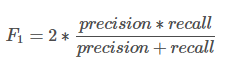
\includegraphics[width=0.3\linewidth]{F1_score} \end{center}

donde:

\begin{center}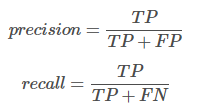
\includegraphics[width=0.25\linewidth]{F1_score_2} \end{center}

La partición inicial train-test, no se tiene que realizar, ya que las
instancias de train y test ya vienen definidas en el dataset de la
competición (ficheros \textbf{train.csv} y \textbf{test.csv}).

A continuación, cargaremos el conjunto de datos de train y test,
nombrando los valores perdidos como \textbf{NA} para que los podamos
tratar más adelante, y mostraremos sus dimensiones.

\begin{Shaded}
\begin{Highlighting}[]
\NormalTok{train <-}\StringTok{ }\KeywordTok{read.csv}\NormalTok{(}\StringTok{"train.csv"}\NormalTok{, }\DataTypeTok{na.strings=}\KeywordTok{c}\NormalTok{(}\StringTok{""}\NormalTok{, }\StringTok{"NA"}\NormalTok{))}
\NormalTok{test <-}\StringTok{ }\KeywordTok{read.csv}\NormalTok{(}\StringTok{"test.csv"}\NormalTok{, }\DataTypeTok{na.strings=}\KeywordTok{c}\NormalTok{(}\StringTok{""}\NormalTok{, }\StringTok{"NA"}\NormalTok{))}
\KeywordTok{dim}\NormalTok{(train)}
\end{Highlighting}
\end{Shaded}

\begin{verbatim}
## [1] 7613    5
\end{verbatim}

\begin{Shaded}
\begin{Highlighting}[]
\KeywordTok{dim}\NormalTok{(test)}
\end{Highlighting}
\end{Shaded}

\begin{verbatim}
## [1] 3263    4
\end{verbatim}

El conjunto de datos de train contiene 7613 instancias y el conjunto de
datos de test contiene 3263 instancias. Cada instancia de estos
conjuntos contiene la siguiente información:

\begin{itemize}
\tightlist
\item
  \textbf{id}: un identificador único para cada tweet.
\item
  \textbf{keyword}: una palabra clave del tweet.
\item
  \textbf{location}: la ubicación desde la que se envió el tweet.
\item
  \textbf{text}: el texto del tweet.
\item
  \textbf{target}: solo en el conjunto de datos de train porqué es la
  variable clase a predecir. Indica si un tweet es sobre un desastre
  real (1) o no (0).
\end{itemize}

\begin{Shaded}
\begin{Highlighting}[]
\KeywordTok{str}\NormalTok{(train, }\DataTypeTok{width =} \DecValTok{85}\NormalTok{, }\DataTypeTok{strict.width =} \StringTok{"cut"}\NormalTok{)}
\end{Highlighting}
\end{Shaded}

\begin{verbatim}
## 'data.frame':    7613 obs. of  5 variables:
##  $ id      : int  1 4 5 6 7 8 10 13 14 15 ...
##  $ keyword : chr  NA NA NA NA ...
##  $ location: chr  NA NA NA NA ...
##  $ text    : chr  "Our Deeds are the Reason of this #earthquake May ALLAH Forgive "..
##  $ target  : int  1 1 1 1 1 1 1 1 1 1 ...
\end{verbatim}

\begin{Shaded}
\begin{Highlighting}[]
\KeywordTok{str}\NormalTok{(test, }\DataTypeTok{width =} \DecValTok{85}\NormalTok{, }\DataTypeTok{strict.width =} \StringTok{"cut"}\NormalTok{)}
\end{Highlighting}
\end{Shaded}

\begin{verbatim}
## 'data.frame':    3263 obs. of  4 variables:
##  $ id      : int  0 2 3 9 11 12 21 22 27 29 ...
##  $ keyword : chr  NA NA NA NA ...
##  $ location: chr  NA NA NA NA ...
##  $ text    : chr  "Just happened a terrible car crash" "Heard about #earthquake is"..
\end{verbatim}

\hypertarget{variable-target}{%
\subsubsection{\texorpdfstring{Variable
\emph{target}}{Variable target}}\label{variable-target}}

Categorizamos la variable a predecir, ya que inicialmente es de tipo
entero, y observamos su distribución.

\begin{Shaded}
\begin{Highlighting}[]
\NormalTok{train}\OperatorTok{$}\NormalTok{target <-}\StringTok{ }\KeywordTok{as.factor}\NormalTok{(}\KeywordTok{ifelse}\NormalTok{(train}\OperatorTok{$}\NormalTok{target }\OperatorTok{==}\StringTok{ }\DecValTok{0}\NormalTok{, }\StringTok{"No"}\NormalTok{, }\StringTok{"Yes"}\NormalTok{))}
\KeywordTok{ggplot}\NormalTok{(train, }\KeywordTok{aes}\NormalTok{(}\DataTypeTok{x=}\NormalTok{target)) }\OperatorTok{+}\StringTok{ }\KeywordTok{geom_bar}\NormalTok{(}\KeywordTok{aes}\NormalTok{(}\DataTypeTok{fill=}\NormalTok{target))}
\end{Highlighting}
\end{Shaded}

\begin{center}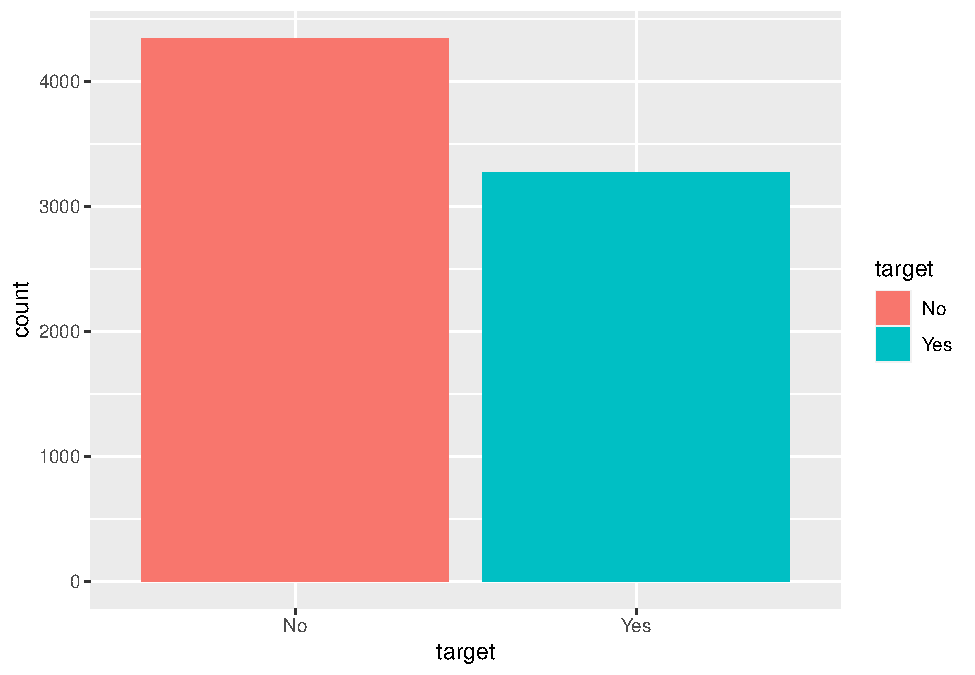
\includegraphics[width=0.7\linewidth]{document_files/figure-latex/unnamed-chunk-6-1} \end{center}

La distribución no está muy sesgada y vemos que hay menos tweets que se
refieren a desastres reales. La distribución de la variable a predecir
está relativamente equilibrada, donde el 43\% de las observaciones son
desastrosas y el 57\% no.

\begin{Shaded}
\begin{Highlighting}[]
\KeywordTok{sum}\NormalTok{(train}\OperatorTok{$}\NormalTok{target }\OperatorTok{==}\StringTok{ "Yes"}\NormalTok{) }\OperatorTok{/}\StringTok{ }\KeywordTok{dim}\NormalTok{(train)[}\DecValTok{1}\NormalTok{] }\OperatorTok{*}\StringTok{ }\DecValTok{100}
\end{Highlighting}
\end{Shaded}

\begin{verbatim}
## [1] 42.96598
\end{verbatim}

\begin{Shaded}
\begin{Highlighting}[]
\KeywordTok{sum}\NormalTok{(train}\OperatorTok{$}\NormalTok{target }\OperatorTok{==}\StringTok{ "No"}\NormalTok{) }\OperatorTok{/}\StringTok{ }\KeywordTok{dim}\NormalTok{(train)[}\DecValTok{1}\NormalTok{] }\OperatorTok{*}\StringTok{ }\DecValTok{100}
\end{Highlighting}
\end{Shaded}

\begin{verbatim}
## [1] 57.03402
\end{verbatim}

Tampoco presenta un problema notable de \emph{desbalanceo de clase}
porqué contamos con muchas muestras del caso minoritario.

\hypertarget{variable-keyword}{%
\subsubsection{\texorpdfstring{Variable
\emph{keyword}}{Variable keyword}}\label{variable-keyword}}

La variable \textbf{keyword} representa una palabra representativa de
cada tweet, se muestran las primeras 10.

\begin{Shaded}
\begin{Highlighting}[]
\NormalTok{train }\OperatorTok\StringTok{ }\KeywordTok{select}\NormalTok{(keyword) }\OperatorTok\StringTok{ }\KeywordTok{unique}\NormalTok{() }\OperatorTok\StringTok{ }\KeywordTok{head}\NormalTok{(}\DecValTok{10}\NormalTok{)}
\end{Highlighting}
\end{Shaded}

\begin{verbatim}
##                 keyword
## 1                  <NA>
## 32               ablaze
## 68             accident
## 103          aftershock
## 137 airplane%20accident
## 172           ambulance
## 210         annihilated
## 244        annihilation
## 273          apocalypse
## 305          armageddon
\end{verbatim}

Ahora veremos si la asociación de cada \textbf{keyword} con un
sentimiento indica una relación con la variable a predecir. Para ello
realizaremos un análisis de sentimientos de cada palabra clave.

\emph{El análisis de sentimientos es una técnica de }Machine
Learning\emph{, basada en el
\href{https://www.kdnuggets.com/2017/02/natural-language-processing-key-terms-explained.html}{procesado
del lenguaje natural}, que pretende obtener información subjetiva de una
serie de textos. Su aplicación es este caso, consiste en resolver si un
tweet es real o no real en relación a un desastre.}

Para ello usaremos los paquetes \textbf{syuzhet}, \textbf{ggcorrplot} y
\textbf{doParallel}.

\begin{itemize}
\tightlist
\item
  \textbf{syuzhet} cuenta con la función \textbf{get\_nrc\_sentiment}
  que calcula la presencia de los diferentes sentimientos dado un
  conjunto de textos. Los parámetros de esta función son:

  \begin{itemize}
  \tightlist
  \item
    \textbf{char\_v}. Un vector de caracteres que en este caso contiene
    todas las palabras clave.
  \item
    \textbf{language}. Define el lenguaje.
  \item
    \textbf{cl}. Para análisis paralelo. Es opcional, pero en este caso
    lo usaremos porqué hay muchas palabras clave.
  \end{itemize}
\item
  \textbf{ggcorrplot} muestra una visualización gráfica de una matriz de
  correlación usando \emph{ggplot2}.
\item
  \textbf{doParallel} proporciona una computación paralela. Los
  parámetros de esta función son:

  \begin{itemize}
  \tightlist
  \item
    \textbf{makePSOCKcluster}. Crea un clúster de sockets paralelos.
  \item
    \textbf{registerDoParallel}. Registra el número de \emph{cores} que
    usará el clúster creado.
  \item
    \textbf{stopCluster}. Detiene la computación paralela.
  \end{itemize}
\end{itemize}

Análisis de correlaciones entre \textbf{keyword} y \textbf{target}:

\begin{Shaded}
\begin{Highlighting}[]
\NormalTok{emocion.df <-}\StringTok{ }\KeywordTok{get_nrc_sentiment}\NormalTok{(}\DataTypeTok{char_v =} \KeywordTok{gsub}\NormalTok{(}\StringTok{"_"}\NormalTok{, }\StringTok{" "}\NormalTok{, train}\OperatorTok{$}\NormalTok{keyword), }
                                \DataTypeTok{language =} \StringTok{"english"}\NormalTok{, }\DataTypeTok{cl=}\NormalTok{cl)}

\NormalTok{emocion.df <-}\StringTok{ }\NormalTok{emocion.df }\OperatorTok\StringTok{ }\KeywordTok{data.frame}\NormalTok{(}\DataTypeTok{target =}\NormalTok{ train}\OperatorTok{$}\NormalTok{target)}
\NormalTok{emocion.df}\OperatorTok{$}\NormalTok{target <-}\StringTok{ }\KeywordTok{as.numeric}\NormalTok{(emocion.df}\OperatorTok{$}\NormalTok{target)}

\KeywordTok{cor}\NormalTok{(emocion.df) }\OperatorTok\StringTok{ }
\StringTok{  }\KeywordTok{ggcorrplot}\NormalTok{(}\DataTypeTok{lab =} \OtherTok{TRUE}\NormalTok{, }
             \DataTypeTok{title =} \StringTok{"Matriz de correlación entre los }\CharTok{\textbackslash{}n}\StringTok{sentimientos de keyword y target"}\NormalTok{,}
             \DataTypeTok{legend.title =} \StringTok{"correlation"}\NormalTok{)}
\end{Highlighting}
\end{Shaded}

\begin{center}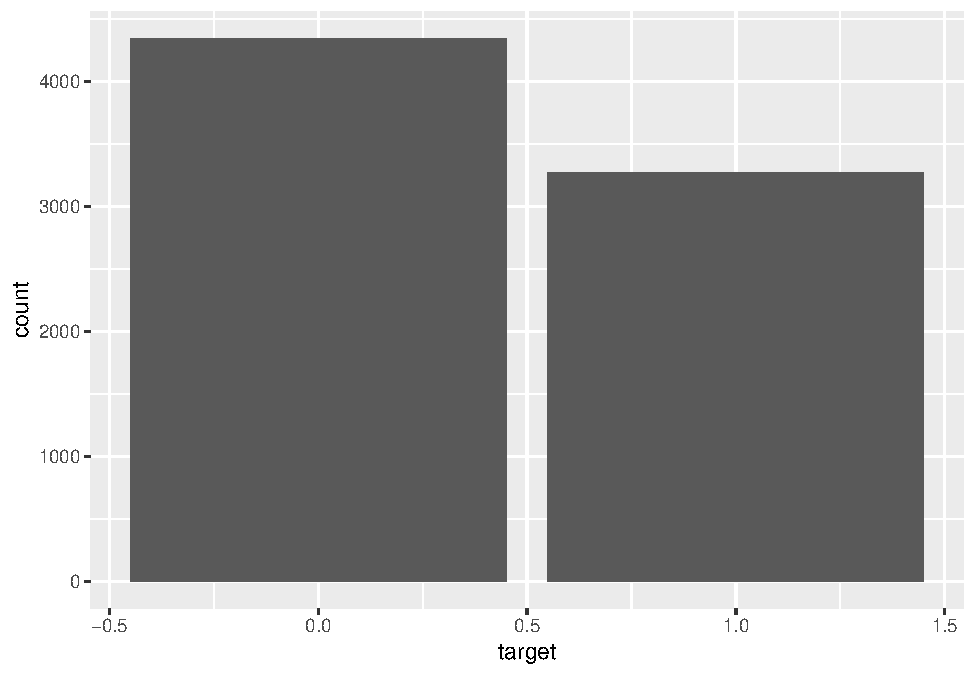
\includegraphics[width=0.7\linewidth]{document_files/figure-latex/unnamed-chunk-10-1} \end{center}

Al observar la matriz de correlaciones, se observa una correlación nula
con cada uno de los sentimientos. Esto hace que esta variable
explicativa no sea buena para hacer una predicción.

\hypertarget{variable-location}{%
\subsubsection{\texorpdfstring{Variable
\emph{location}}{Variable location}}\label{variable-location}}

La variable \textbf{location} representa la ubicación desde donde se
generaron los tweets, se muestran las primeras 10.

\begin{Shaded}
\begin{Highlighting}[]
\NormalTok{train }\OperatorTok\StringTok{ }\KeywordTok{select}\NormalTok{(location) }\OperatorTok\StringTok{ }\KeywordTok{unique}\NormalTok{() }\OperatorTok\StringTok{ }\KeywordTok{head}\NormalTok{(}\DecValTok{10}\NormalTok{)}
\end{Highlighting}
\end{Shaded}

\begin{verbatim}
##                         location
## 1                           <NA>
## 32                    Birmingham
## 33 Est. September 2012 - Bristol
## 34                        AFRICA
## 35              Philadelphia, PA
## 36                    London, UK
## 37                      Pretoria
## 38                  World Wide!!
## 40                Paranaque City
## 41                Live On Webcam
\end{verbatim}

\begin{Shaded}
\begin{Highlighting}[]
\KeywordTok{count}\NormalTok{(train }\OperatorTok\StringTok{ }\KeywordTok{select}\NormalTok{(location) }\OperatorTok\StringTok{ }\KeywordTok{unique}\NormalTok{())}
\end{Highlighting}
\end{Shaded}

\begin{verbatim}
##      n
## 1 3342
\end{verbatim}

En total hay 3342 ubicaciones. A continuación, mostramos las ubicaciones
más frecuentes:

\begin{Shaded}
\begin{Highlighting}[]
\NormalTok{location.freq <-}\StringTok{ }\KeywordTok{table}\NormalTok{(}\KeywordTok{unlist}\NormalTok{(train }\OperatorTok\StringTok{ }\KeywordTok{select}\NormalTok{(location)))}
\NormalTok{location.freq[}\KeywordTok{which}\NormalTok{(location.freq }\OperatorTok{>}\StringTok{ }\DecValTok{10}\NormalTok{)]}
\end{Highlighting}
\end{Shaded}

\begin{verbatim}
## 
##         Australia        California   California, USA            Canada 
##                18                17                15                29 
##           Chicago       Chicago, IL             Earth        Everywhere 
##                11                18                11                15 
##           Florida             India         Indonesia           Ireland 
##                14                24                13                12 
##             Kenya            London       Los Angeles   Los Angeles, CA 
##                20                45                13                26 
##            Mumbai          New York      New York, NY           Nigeria 
##                22                71                15                28 
##               NYC     San Francisco San Francisco, CA           Seattle 
##                12                14                11                11 
##           Toronto                UK    United Kingdom     United States 
##                12                27                14                50 
##               USA  Washington, D.C.    Washington, DC         Worldwide 
##               104                13                21                19
\end{verbatim}

\begin{Shaded}
\begin{Highlighting}[]
\KeywordTok{barplot}\NormalTok{(location.freq[}\KeywordTok{which}\NormalTok{(location.freq}\OperatorTok{>}\DecValTok{10}\NormalTok{)], }\DataTypeTok{las =} \DecValTok{2}\NormalTok{,  }
        \DataTypeTok{ylab =} \StringTok{"Frequency"}\NormalTok{)}
\end{Highlighting}
\end{Shaded}

\begin{center}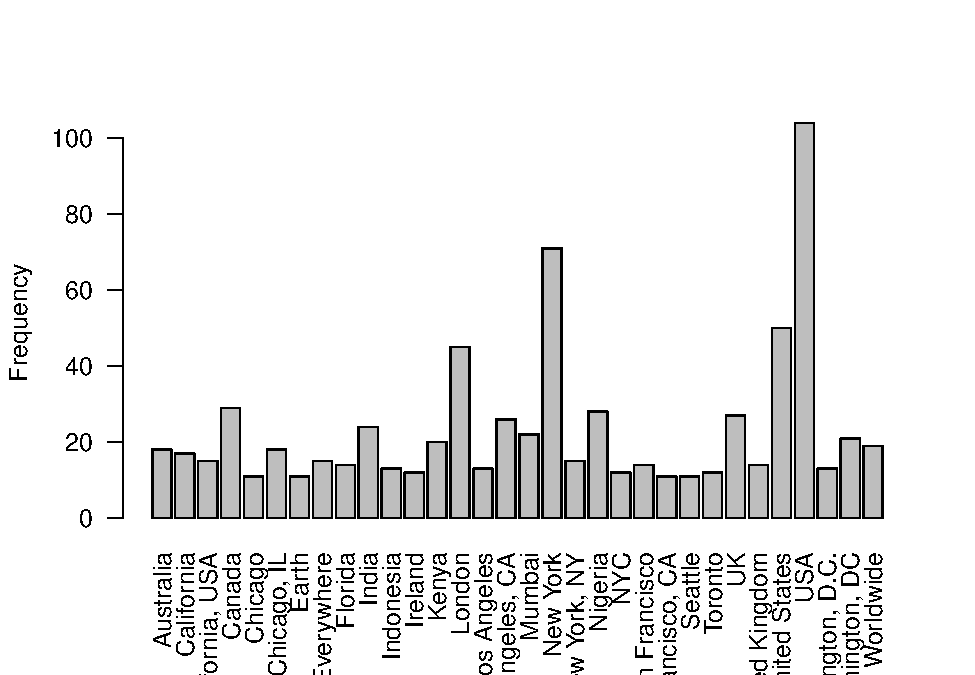
\includegraphics[width=0.7\linewidth]{document_files/figure-latex/unnamed-chunk-13-1} \end{center}

Del total de ubicaciones (3342), la mayoría de ellas cuenta con menos de
10 observaciones. Esto hace que esta variable explicativa tampoco sea
buena para hacer una predicción.

\hypertarget{variable-text}{%
\subsubsection{\texorpdfstring{Variable
\emph{text}}{Variable text}}\label{variable-text}}

Hemos considerado que las variables explicativas \textbf{keyword} y
\textbf{location} no son buenas para hacer una predicción, así que nos
centraremos en la variable \textbf{text}.

Llegados a este punto unimos los conjuntos de train y test (\emph{7613 +
3263 observaciones}) para poder extraer los sentimientos más adelante.

\begin{Shaded}
\begin{Highlighting}[]
\NormalTok{complete_df <-}\StringTok{ }\KeywordTok{bind_rows}\NormalTok{(train, test)}
\KeywordTok{dim}\NormalTok{(complete_df)}
\end{Highlighting}
\end{Shaded}

\begin{verbatim}
## [1] 10876     5
\end{verbatim}

Echamos un vistazo más de cerca a las variables del nuevo conjunto de
datos \textbf{complete\_df}.

\begin{Shaded}
\begin{Highlighting}[]
\KeywordTok{summary}\NormalTok{(complete_df)}
\end{Highlighting}
\end{Shaded}

\begin{verbatim}
##        id          keyword            location             text          
##  Min.   :    0   Length:10876       Length:10876       Length:10876      
##  1st Qu.: 2719   Class :character   Class :character   Class :character  
##  Median : 5438   Mode  :character   Mode  :character   Mode  :character  
##  Mean   : 5438                                                           
##  3rd Qu.: 8156                                                           
##  Max.   :10875                                                           
##   target    
##  No  :4342  
##  Yes :3271  
##  NA's:3263  
##             
##             
## 
\end{verbatim}

La variable \textbf{id} es solo un identificador único y la
eliminaremos.

\begin{Shaded}
\begin{Highlighting}[]
\NormalTok{complete_df}\OperatorTok{$}\NormalTok{id <-}\StringTok{ }\OtherTok{NULL}
\end{Highlighting}
\end{Shaded}

Observamos si existen valores perdidos.

\begin{Shaded}
\begin{Highlighting}[]
\KeywordTok{colSums}\NormalTok{(}\KeywordTok{sapply}\NormalTok{(complete_df, is.na))}
\end{Highlighting}
\end{Shaded}

\begin{verbatim}
##  keyword location     text   target 
##       87     3638        0     3263
\end{verbatim}

Las variables explicativas \textbf{keyword} y \textbf{location}
contienen valores perdidos. Sobretodo hay una gran cantidad de tweets,
para los cuales falta su ubicación. No existen valores perdidos para la
variable explicativa \textbf{text}, tampoco para la variable a predecir
\textbf{target}. Los 3263 valores perdidos de la variable a predecir
provienen del conjunto de datos de test. Nos ocuparemos de los valores
perdidos más adelante.

Parece que la variable explicativa \textbf{text} es una buena elección
para una buena predicción y basaremos los siguientes pasos en ella.

\hypertarget{procesamiento-de-texto}{%
\subsection{Procesamiento de texto}\label{procesamiento-de-texto}}

Como en todo procesamiento de lenguaje natural, realizaremos el
procesamiento de un conjunto de textos. En este caso realizaremos un
procesamiento de los textos de los tweets y los prepararemos para el
modelado. Comencemos por crear un corpus de los mensajes de texto de los
tweets. Para ello usaremos la función \textbf{Corpus} del paquete
\textbf{tm}, que creará nuestro corpus a partir de un vector de textos.
La función \textbf{VectorSource} interpretará cada mensaje de texto de
los tweets como un elemento del vector de textos.

\emph{Un corpus lingüístico se define como ``un conjunto de textos de un
mismo origen'' y que tiene por función recopilar un conjunto de textos.
El uso de un corpus lingüístico nos permitirá obtener información de las
palabras utilizadas con más o menor frecuencia.}

\begin{Shaded}
\begin{Highlighting}[]
\NormalTok{myCorpus <-}\StringTok{ }\KeywordTok{Corpus}\NormalTok{(}\KeywordTok{VectorSource}\NormalTok{(complete_df}\OperatorTok{$}\NormalTok{text))}
\end{Highlighting}
\end{Shaded}

Durante el procesamiento de texto seguiremos la transformación de un
mensaje de tweet específico para ver como se modifica a medida que
avanzamos en el procesamiento de texto. Este mensaje es:

\begin{Shaded}
\begin{Highlighting}[]
\KeywordTok{paste0}\NormalTok{(myCorpus[[}\DecValTok{400}\NormalTok{]])}
\end{Highlighting}
\end{Shaded}

\begin{verbatim}
## [1] "Jewish leaders prayed at the hospital where a Palestinian family is being treated after arson http://t.co/Wf8iTK2KVx via @HuffPostRelig"
\end{verbatim}

Dividimos el procesamiento de texto en 7 pasos.

\begin{enumerate}
\def\labelenumi{\arabic{enumi}.}
\tightlist
\item
  Eliminar enlaces.
\end{enumerate}

\begin{Shaded}
\begin{Highlighting}[]
\NormalTok{removeURL <-}\StringTok{ }\ControlFlowTok{function}\NormalTok{(x) }\KeywordTok{gsub}\NormalTok{(}\StringTok{"http[^[:space:]]*"}\NormalTok{, }\StringTok{""}\NormalTok{, x)  }
\NormalTok{myCorpus <-}\StringTok{ }\KeywordTok{tm_map}\NormalTok{(myCorpus, }\KeywordTok{content_transformer}\NormalTok{(removeURL))}
\KeywordTok{paste0}\NormalTok{(myCorpus[[}\DecValTok{400}\NormalTok{]])}
\end{Highlighting}
\end{Shaded}

\begin{verbatim}
## [1] "Jewish leaders prayed at the hospital where a Palestinian family is being treated after arson  via @HuffPostRelig"
\end{verbatim}

Hemos eliminado: \emph{\url{http://t.co/Wf8iTK2KVx}}.

La función \textbf{gsub} busca y reemplaza desde la primera hasta todas
las coincidencias de un patrón (que normalmente representa una
\emph{regular expression}). La función \textbf{tm\_map} es la encargada
de aplicar las diferentes transformaciones de los textos al corpus
creado.

\begin{enumerate}
\def\labelenumi{\arabic{enumi}.}
\setcounter{enumi}{1}
\tightlist
\item
  Convertir a minúsculas.
\end{enumerate}

\begin{Shaded}
\begin{Highlighting}[]
\NormalTok{myCorpus <-}\StringTok{ }\KeywordTok{tm_map}\NormalTok{(myCorpus, }\KeywordTok{content_transformer}\NormalTok{(stri_trans_tolower))}
\KeywordTok{paste0}\NormalTok{(myCorpus[[}\DecValTok{400}\NormalTok{]])}
\end{Highlighting}
\end{Shaded}

\begin{verbatim}
## [1] "jewish leaders prayed at the hospital where a palestinian family is being treated after arson  via @huffpostrelig"
\end{verbatim}

\begin{enumerate}
\def\labelenumi{\arabic{enumi}.}
\setcounter{enumi}{2}
\tightlist
\item
  Eliminar los nombres de usuario.
\end{enumerate}

\begin{Shaded}
\begin{Highlighting}[]
\NormalTok{removeUsername <-}\StringTok{ }\ControlFlowTok{function}\NormalTok{(x) }\KeywordTok{gsub}\NormalTok{(}\StringTok{"@[^[:space:]]*"}\NormalTok{, }\StringTok{""}\NormalTok{, x)  }
\NormalTok{myCorpus <-}\StringTok{ }\KeywordTok{tm_map}\NormalTok{(myCorpus, }\KeywordTok{content_transformer}\NormalTok{(removeUsername))}
\KeywordTok{paste0}\NormalTok{(myCorpus[[}\DecValTok{400}\NormalTok{]])}
\end{Highlighting}
\end{Shaded}

\begin{verbatim}
## [1] "jewish leaders prayed at the hospital where a palestinian family is being treated after arson  via "
\end{verbatim}

Hemos eliminado: \emph{@huffpostrelig}.

\begin{enumerate}
\def\labelenumi{\arabic{enumi}.}
\setcounter{enumi}{3}
\tightlist
\item
  Eliminar todo excepto el idioma y el espacio en inglés.
\end{enumerate}

\begin{Shaded}
\begin{Highlighting}[]
\NormalTok{removeNumPunct <-}\StringTok{ }\ControlFlowTok{function}\NormalTok{(x) }\KeywordTok{gsub}\NormalTok{(}\StringTok{"[^[:alpha:][:space:]]*"}\NormalTok{, }\StringTok{""}\NormalTok{, x)   }
\NormalTok{myCorpus <-}\StringTok{ }\KeywordTok{tm_map}\NormalTok{(myCorpus, }\KeywordTok{content_transformer}\NormalTok{(removeNumPunct))}
\KeywordTok{paste0}\NormalTok{(myCorpus[[}\DecValTok{400}\NormalTok{]])}
\end{Highlighting}
\end{Shaded}

\begin{verbatim}
## [1] "jewish leaders prayed at the hospital where a palestinian family is being treated after arson  via "
\end{verbatim}

No se observan cambios en en ejemplo.

\begin{enumerate}
\def\labelenumi{\arabic{enumi}.}
\setcounter{enumi}{4}
\tightlist
\item
  Eliminar palabras irrelevantes (eliminación de redundancias).
\end{enumerate}

\begin{Shaded}
\begin{Highlighting}[]
\NormalTok{myStopWords <-}\StringTok{ }\KeywordTok{c}\NormalTok{((}\KeywordTok{stopwords}\NormalTok{(}\StringTok{'english'}\NormalTok{)), }
         \KeywordTok{c}\NormalTok{(}\StringTok{"really"}\NormalTok{, }\StringTok{"tweets"}\NormalTok{, }\StringTok{"saw"}\NormalTok{, }\StringTok{"just"}\NormalTok{, }\StringTok{"feel"}\NormalTok{, }\StringTok{"may"}\NormalTok{, }\StringTok{"us"}\NormalTok{, }\StringTok{"rt"}\NormalTok{, }\StringTok{"every"}\NormalTok{, }\StringTok{"one"}\NormalTok{,}
           \StringTok{"amp"}\NormalTok{, }\StringTok{"like"}\NormalTok{, }\StringTok{"will"}\NormalTok{, }\StringTok{"got"}\NormalTok{, }\StringTok{"new"}\NormalTok{, }\StringTok{"can"}\NormalTok{, }\StringTok{"still"}\NormalTok{, }\StringTok{"back"}\NormalTok{, }\StringTok{"top"}\NormalTok{, }\StringTok{"much"}\NormalTok{,}
           \StringTok{"near"}\NormalTok{, }\StringTok{"im"}\NormalTok{, }\StringTok{"see"}\NormalTok{, }\StringTok{"via"}\NormalTok{, }\StringTok{"get"}\NormalTok{, }\StringTok{"now"}\NormalTok{, }\StringTok{"come"}\NormalTok{, }\StringTok{"oil"}\NormalTok{, }\StringTok{"let"}\NormalTok{, }\StringTok{"god"}\NormalTok{, }\StringTok{"want"}\NormalTok{,}
           \StringTok{"pm"}\NormalTok{, }\StringTok{"last"}\NormalTok{, }\StringTok{"hope"}\NormalTok{, }\StringTok{"since"}\NormalTok{, }\StringTok{"everyone"}\NormalTok{, }\StringTok{"food"}\NormalTok{, }\StringTok{"content"}\NormalTok{, }\StringTok{"always"}\NormalTok{, }\StringTok{"th"}\NormalTok{,}
           \StringTok{"full"}\NormalTok{, }\StringTok{"found"}\NormalTok{, }\StringTok{"dont"}\NormalTok{, }\StringTok{"look"}\NormalTok{, }\StringTok{"cant"}\NormalTok{, }\StringTok{"mh"}\NormalTok{, }\StringTok{"lol"}\NormalTok{, }\StringTok{"set"}\NormalTok{, }\StringTok{"old"}\NormalTok{, }\StringTok{"service"}\NormalTok{,}
           \StringTok{"city"}\NormalTok{, }\StringTok{"home"}\NormalTok{, }\StringTok{"live"}\NormalTok{, }\StringTok{"night"}\NormalTok{, }\StringTok{"news"}\NormalTok{, }\StringTok{"say"}\NormalTok{, }\StringTok{"video"}\NormalTok{, }\StringTok{"people"}\NormalTok{, }\StringTok{"ill"}\NormalTok{, }
           \StringTok{"way"}\NormalTok{,  }\StringTok{"please"}\NormalTok{, }\StringTok{"years"}\NormalTok{, }\StringTok{"take"}\NormalTok{, }\StringTok{"homes"}\NormalTok{, }\StringTok{"read"}\NormalTok{, }\StringTok{"man"}\NormalTok{, }\StringTok{"next"}\NormalTok{, }\StringTok{"cross"}\NormalTok{, }
           \StringTok{"boy"}\NormalTok{, }\StringTok{"bad"}\NormalTok{, }\StringTok{"ass"}\NormalTok{))}

\NormalTok{myCorpus <-}\StringTok{ }\KeywordTok{tm_map}\NormalTok{(myCorpus, removeWords, myStopWords) }
\KeywordTok{paste0}\NormalTok{(myCorpus[[}\DecValTok{400}\NormalTok{]])}
\end{Highlighting}
\end{Shaded}

\begin{verbatim}
## [1] "jewish leaders prayed   hospital   palestinian family   treated  arson   "
\end{verbatim}

Hemos eliminado: at the where a is being after via.

Las palabras irrelevantes que hemos eliminado se denominan \emph{stop
words o palabras vacías}. Cada idioma tiene sus propias palabras vacías.
Como los textos están en inglés hemos eliminado los \emph{stop words}
que pertenecen al inglés usando la función \textbf{stopwords}, además
hemos añadido aleatóriamente alguna de las palabras vacías más usadas en
los mensajes de texto de los tweets (ver
\url{https://techland.time.com/2009/06/08/the-500-most-frequently-used-words-on-twitter/}).

\emph{Las stop words o palabras vacías son todas aquellas palabras que
carecen de un significado por si solas. Suelen ser artículos,
preposiciones, conjunciones, pronombres, etc.}

\begin{enumerate}
\def\labelenumi{\arabic{enumi}.}
\setcounter{enumi}{5}
\tightlist
\item
  Eliminar palabras de una sola letra.
\end{enumerate}

\begin{Shaded}
\begin{Highlighting}[]
\NormalTok{removeSingle <-}\StringTok{ }\ControlFlowTok{function}\NormalTok{(x) }\KeywordTok{gsub}\NormalTok{(}\StringTok{" . "}\NormalTok{, }\StringTok{" "}\NormalTok{, x)   }
\NormalTok{myCorpus <-}\StringTok{ }\KeywordTok{tm_map}\NormalTok{(myCorpus, }\KeywordTok{content_transformer}\NormalTok{(removeSingle))}
\KeywordTok{paste0}\NormalTok{(myCorpus[[}\DecValTok{400}\NormalTok{]])}
\end{Highlighting}
\end{Shaded}

\begin{verbatim}
## [1] "jewish leaders prayed hospital palestinian family treated  arson "
\end{verbatim}

No se observan cambios en en ejemplo.

\begin{enumerate}
\def\labelenumi{\arabic{enumi}.}
\setcounter{enumi}{6}
\tightlist
\item
  Eliminar espacios en blanco adicionales.
\end{enumerate}

\begin{Shaded}
\begin{Highlighting}[]
\NormalTok{myCorpus <-}\StringTok{ }\KeywordTok{tm_map}\NormalTok{(myCorpus, stripWhitespace)}
\KeywordTok{paste0}\NormalTok{(myCorpus[[}\DecValTok{400}\NormalTok{]])}
\end{Highlighting}
\end{Shaded}

\begin{verbatim}
## [1] "jewish leaders prayed hospital palestinian family treated arson "
\end{verbatim}

Terminamos con el procesamiento de texto. A continuación, crearemos dos
\emph{Term Document Matrix} (matriz que describe la frecuencia de las
palabras que se producen en una colección de textos) para un análisis de
sentimientos más detallado. Usaremos la función
\textbf{TermDocumentMatrix} y dividiremos el corpus en dos, según el
número de elementos de los conjuntos de datos train y test. Recordamos
que el conjunto de datos de train contiene 7613 observaciones, y el
conjunto de datos de test contiene 3263 observaciones. El parámetro
\textbf{control} evalúa cada texto de la matriz, específicamente se
evaluaran todas las palabras de cada texto (no aplicamos ningún filtro).

\begin{Shaded}
\begin{Highlighting}[]
\NormalTok{train_tdm <-}\StringTok{ }\KeywordTok{TermDocumentMatrix}\NormalTok{(myCorpus[}\DecValTok{1}\OperatorTok{:}\DecValTok{7613}\NormalTok{], }
                                \DataTypeTok{control=} \KeywordTok{list}\NormalTok{(}\DataTypeTok{wordLengths=} \KeywordTok{c}\NormalTok{(}\DecValTok{1}\NormalTok{, }\OtherTok{Inf}\NormalTok{)))}
\NormalTok{test_tdm <-}\StringTok{ }\KeywordTok{TermDocumentMatrix}\NormalTok{(myCorpus[}\DecValTok{7614}\OperatorTok{:}\DecValTok{10876}\NormalTok{], }
                               \DataTypeTok{control=} \KeywordTok{list}\NormalTok{(}\DataTypeTok{wordLengths=} \KeywordTok{c}\NormalTok{(}\DecValTok{1}\NormalTok{, }\OtherTok{Inf}\NormalTok{)))}
\NormalTok{train_tdm}
\end{Highlighting}
\end{Shaded}

\begin{verbatim}
## <<TermDocumentMatrix (terms: 14825, documents: 7613)>>
## Non-/sparse entries: 58707/112804018
## Sparsity           : 100%
## Maximal term length: 49
## Weighting          : term frequency (tf)
\end{verbatim}

\begin{Shaded}
\begin{Highlighting}[]
\NormalTok{test_tdm}
\end{Highlighting}
\end{Shaded}

\begin{verbatim}
## <<TermDocumentMatrix (terms: 8966, documents: 3263)>>
## Non-/sparse entries: 25434/29230624
## Sparsity           : 100%
## Maximal term length: 35
## Weighting          : term frequency (tf)
\end{verbatim}

La matriz para los datos de train contiene 14825 palabras y la matriz
para los datos de test contiene 8966 palabras. Utilizaremos las matrices
para ver las palabras más utilizadas en los tweets y predecir a partir
de ellas.

\hypertarget{palabras-muxe1s-frecuentes}{%
\subsection{Palabras más frecuentes}\label{palabras-muxe1s-frecuentes}}

\begin{itemize}
\tightlist
\item
  Palabras más frecuentes en los datos de train.
\end{itemize}

\begin{Shaded}
\begin{Highlighting}[]
\NormalTok{train.term.freq <-}\StringTok{ }\KeywordTok{rowSums}\NormalTok{(}\KeywordTok{as.matrix}\NormalTok{(train_tdm))}
\NormalTok{train.term.freq <-}\StringTok{ }\KeywordTok{subset}\NormalTok{(train.term.freq, train.term.freq }\OperatorTok{>}\StringTok{ }\DecValTok{60}\NormalTok{)}
\NormalTok{freq_train_df <-}\StringTok{ }\KeywordTok{data.frame}\NormalTok{(}\DataTypeTok{term =} \KeywordTok{names}\NormalTok{(train.term.freq), }\DataTypeTok{freq=}\NormalTok{ train.term.freq)}
\KeywordTok{head}\NormalTok{(freq_train_df[}\KeywordTok{order}\NormalTok{(}\OperatorTok{-}\NormalTok{freq_train_df}\OperatorTok{$}\NormalTok{freq), ])}
\end{Highlighting}
\end{Shaded}

\begin{verbatim}
##                term freq
## fire           fire  250
## emergency emergency  157
## disaster   disaster  152
## police       police  140
## time           time  125
## body           body  124
\end{verbatim}

\begin{Shaded}
\begin{Highlighting}[]
\KeywordTok{ggplot}\NormalTok{(freq_train_df, }\KeywordTok{aes}\NormalTok{(}\KeywordTok{reorder}\NormalTok{(term, freq), freq)) }\OperatorTok{+}\StringTok{ }\KeywordTok{theme_bw}\NormalTok{() }\OperatorTok{+}\StringTok{ }
\StringTok{  }\KeywordTok{geom_bar}\NormalTok{(}\DataTypeTok{stat =} \StringTok{"identity"}\NormalTok{)  }\OperatorTok{+}\StringTok{ }
\StringTok{  }\KeywordTok{coord_flip}\NormalTok{() }\OperatorTok{+}\StringTok{ }
\StringTok{  }\KeywordTok{theme}\NormalTok{(}\DataTypeTok{axis.text.y =} \KeywordTok{element_text}\NormalTok{(}\DataTypeTok{size=}\DecValTok{7}\NormalTok{))}
\end{Highlighting}
\end{Shaded}

\begin{center}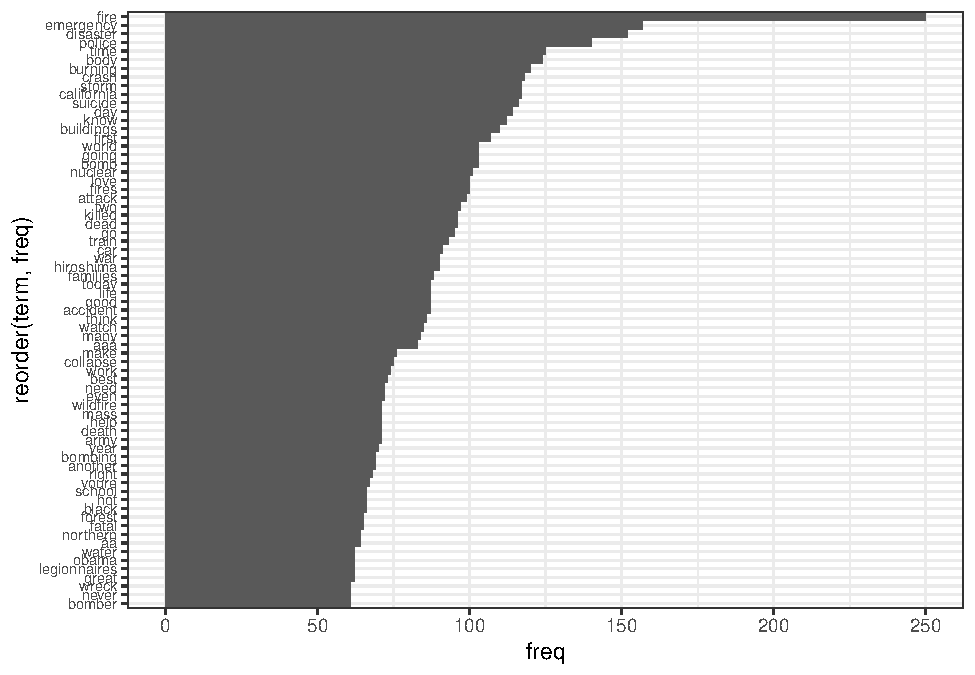
\includegraphics[width=0.7\linewidth]{document_files/figure-latex/unnamed-chunk-28-1} \end{center}

\begin{itemize}
\tightlist
\item
  Palabras más frecuentes en los datos de test
\end{itemize}

\begin{Shaded}
\begin{Highlighting}[]
\NormalTok{test.term.freq <-}\StringTok{ }\KeywordTok{rowSums}\NormalTok{(}\KeywordTok{as.matrix}\NormalTok{(test_tdm))}
\NormalTok{test.term.freq <-}\StringTok{ }\KeywordTok{subset}\NormalTok{(test.term.freq, test.term.freq }\OperatorTok{>}\StringTok{ }\DecValTok{60}\NormalTok{)}
\NormalTok{freq_test_df <-}\StringTok{ }\KeywordTok{data.frame}\NormalTok{(}\DataTypeTok{term =} \KeywordTok{names}\NormalTok{(test.term.freq), }\DataTypeTok{freq=}\NormalTok{ test.term.freq)}
\NormalTok{freq_test_df[}\KeywordTok{order}\NormalTok{(}\OperatorTok{-}\NormalTok{freq_test_df}\OperatorTok{$}\NormalTok{freq), ]}
\end{Highlighting}
\end{Shaded}

\begin{verbatim}
##                term freq
## fire           fire  107
## emergency emergency   68
## attack       attack   63
\end{verbatim}

\begin{Shaded}
\begin{Highlighting}[]
\KeywordTok{ggplot}\NormalTok{(freq_test_df, }\KeywordTok{aes}\NormalTok{(}\KeywordTok{reorder}\NormalTok{(term, freq), freq)) }\OperatorTok{+}\StringTok{ }\KeywordTok{theme_bw}\NormalTok{() }\OperatorTok{+}\StringTok{ }
\StringTok{  }\KeywordTok{geom_bar}\NormalTok{(}\DataTypeTok{stat =} \StringTok{"identity"}\NormalTok{)  }\OperatorTok{+}\StringTok{ }
\StringTok{  }\KeywordTok{coord_flip}\NormalTok{() }\OperatorTok{+}\StringTok{ }
\StringTok{  }\KeywordTok{theme}\NormalTok{(}\DataTypeTok{axis.text.y =} \KeywordTok{element_text}\NormalTok{(}\DataTypeTok{size=}\DecValTok{7}\NormalTok{))}
\end{Highlighting}
\end{Shaded}

\begin{center}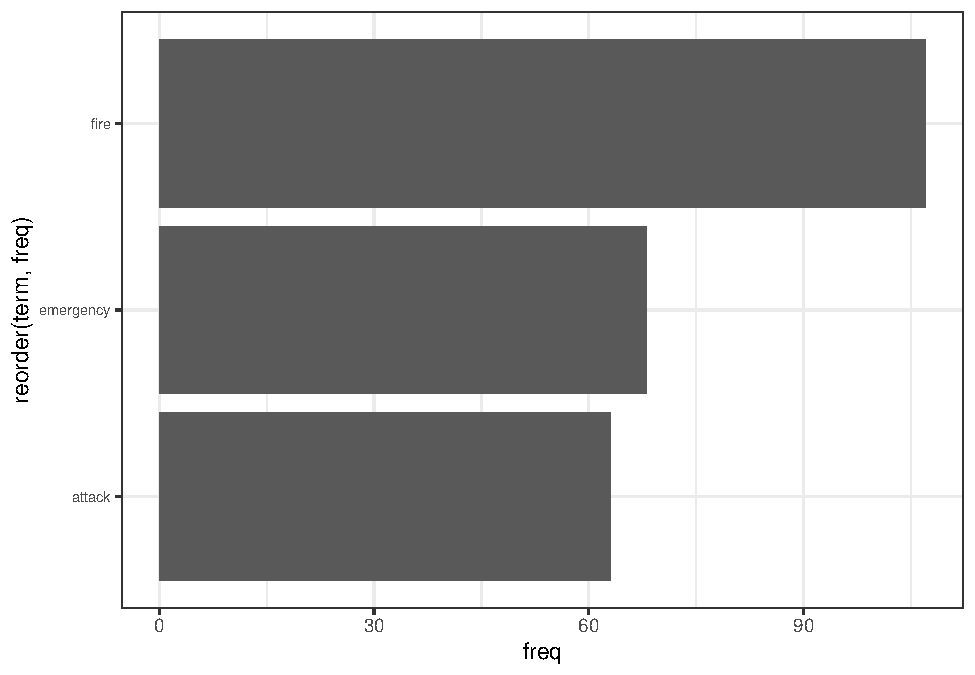
\includegraphics[width=0.5\linewidth]{document_files/figure-latex/unnamed-chunk-29-1} \end{center}

Las palabras \emph{``fire''}, \emph{``attack''} y \emph{``emergency''}
aparecen con alta frecuencia tanto en el conjunto de train como en el
conjunto de test. Estas palabras son muy útiles para predecir un
desastre real.

\hypertarget{modelado}{%
\subsection{Modelado}\label{modelado}}

Para la construcción de modelos, necesitamos construir una \emph{Term
Document Matrix} donde cada fila represente un texto y cada palabra
única esté representada por una columna. Comencemos construyendo la
matriz para nuestro corpus completo.

\begin{Shaded}
\begin{Highlighting}[]
\NormalTok{complete.tdm <-}\StringTok{ }\KeywordTok{TermDocumentMatrix}\NormalTok{(myCorpus, }\DataTypeTok{control=} \KeywordTok{list}\NormalTok{(}\DataTypeTok{wordLengths=} \KeywordTok{c}\NormalTok{(}\DecValTok{4}\NormalTok{, }\OtherTok{Inf}\NormalTok{)))}
\NormalTok{complete.term.matrix <-}\StringTok{ }\KeywordTok{as.matrix}\NormalTok{(}\KeywordTok{t}\NormalTok{(complete.tdm))}
\KeywordTok{dim}\NormalTok{(complete.term.matrix)}
\end{Highlighting}
\end{Shaded}

\begin{verbatim}
## [1] 10876 16891
\end{verbatim}

Podemos ver que es una matriz dispersa con 10876 textos, es decir,
tweets y 16880 palabras. Además, se generan algunos casos incompletos,
que necesitaremos manejar antes de continuar con la construcción del
modelo.

Sin embargo, si intentamos convertir esto para usar esta matriz para la
construcción del modelo, es posible que no podamos entrenar nuestro
modelo debido a restricciones computacionales. Necesitamos reducir la
dimensión/características de la matriz.

Primero tratamos los casos incompletos.

\begin{Shaded}
\begin{Highlighting}[]
\NormalTok{incomplete.cases <-}\StringTok{ }\KeywordTok{which}\NormalTok{(}\OperatorTok{!}\KeywordTok{complete.cases}\NormalTok{(complete.term.matrix))}
\NormalTok{complete.term.matrix[incomplete.cases,] <-}\StringTok{ }\KeywordTok{rep}\NormalTok{(}\FloatTok{0.0}\NormalTok{, }\KeywordTok{ncol}\NormalTok{(complete.term.matrix))}
\end{Highlighting}
\end{Shaded}

\begin{Shaded}
\begin{Highlighting}[]
\NormalTok{complete_irlba <-}\StringTok{ }\KeywordTok{irlba}\NormalTok{(}\KeywordTok{t}\NormalTok{(complete.term.matrix), }\DataTypeTok{nv =} \DecValTok{150}\NormalTok{, }\DataTypeTok{maxit =} \DecValTok{600}\NormalTok{)}
\NormalTok{complete_irlba}\OperatorTok{$}\NormalTok{v[}\DecValTok{1}\OperatorTok{:}\DecValTok{10}\NormalTok{, }\DecValTok{1}\OperatorTok{:}\DecValTok{5}\NormalTok{]}
\end{Highlighting}
\end{Shaded}

\begin{verbatim}
##               [,1]          [,2]          [,3]          [,4]          [,5]
##  [1,] -0.000462870 -0.0003461531  9.263917e-06  1.074148e-04 -0.0006025571
##  [2,] -0.039611815  0.0191637843 -4.631903e-03 -4.704284e-03  0.0075975914
##  [3,] -0.002804300  0.0004191885 -8.592254e-06 -8.570421e-06 -0.0017859899
##  [4,] -0.006221545 -0.0006966814 -2.384731e-03 -2.622132e-04 -0.0034957244
##  [5,] -0.002844704  0.0003113251  1.691928e-04  2.684031e-05 -0.0016029824
##  [6,] -0.043686430  0.0177778044 -6.819700e-03 -4.737299e-03  0.0053901935
##  [7,] -0.010115221 -0.0248025873 -1.819646e-02 -2.408506e-04 -0.0006175213
##  [8,] -0.035196096  0.0178217283 -4.374870e-03 -4.425091e-03  0.0100228792
##  [9,] -0.009139736  0.0007828903 -4.421149e-06  2.046801e-04 -0.0070461856
## [10,] -0.001539314 -0.0001940795 -9.137939e-06  4.200374e-05 -0.0012366532
\end{verbatim}

\begin{Shaded}
\begin{Highlighting}[]
\NormalTok{complete.svd <-}\StringTok{ }\KeywordTok{data.frame}\NormalTok{(}\DataTypeTok{target =}\NormalTok{ complete_df}\OperatorTok{$}\NormalTok{target, complete_irlba}\OperatorTok{$}\NormalTok{v)}
\NormalTok{train.df <-}\StringTok{ }\NormalTok{complete.svd[}\DecValTok{1}\OperatorTok{:}\DecValTok{7613}\NormalTok{, ]}
\NormalTok{test.df <-}\StringTok{ }\NormalTok{complete.svd[}\DecValTok{7614}\OperatorTok{:}\DecValTok{10876}\NormalTok{, }\DecValTok{-1}\NormalTok{]}
\KeywordTok{dim}\NormalTok{(train.df)}
\end{Highlighting}
\end{Shaded}

\begin{verbatim}
## [1] 7613  151
\end{verbatim}

\begin{Shaded}
\begin{Highlighting}[]
\KeywordTok{dim}\NormalTok{(test.df)}
\end{Highlighting}
\end{Shaded}

\begin{verbatim}
## [1] 3263  150
\end{verbatim}

\begin{Shaded}
\begin{Highlighting}[]
\KeywordTok{names}\NormalTok{(train.df) <-}\StringTok{ }\KeywordTok{make.names}\NormalTok{(}\KeywordTok{names}\NormalTok{(train.df))}
\KeywordTok{names}\NormalTok{(test.df) <-}\StringTok{ }\KeywordTok{make.names}\NormalTok{(}\KeywordTok{names}\NormalTok{(test.df))}
\end{Highlighting}
\end{Shaded}

\begin{Shaded}
\begin{Highlighting}[]
\KeywordTok{set.seed}\NormalTok{(}\DecValTok{123}\NormalTok{)}
\NormalTok{cv.folds <-}\StringTok{ }\KeywordTok{createMultiFolds}\NormalTok{(train.df}\OperatorTok{$}\NormalTok{target, }\DataTypeTok{k=}\DecValTok{5}\NormalTok{, }\DataTypeTok{times=}\DecValTok{3}\NormalTok{)}
\NormalTok{cv.cntrl <-}\StringTok{ }\KeywordTok{trainControl}\NormalTok{(}\DataTypeTok{method =} \StringTok{"repeatecv"}\NormalTok{, }\DataTypeTok{number =} \DecValTok{5}\NormalTok{,}
                         \DataTypeTok{index =}\NormalTok{ cv.folds, }\DataTypeTok{allowParallel =} \OtherTok{TRUE}\NormalTok{, }\DataTypeTok{returnResamp=}\StringTok{"final"}\NormalTok{,}
                         \DataTypeTok{verboseIter=}\OtherTok{FALSE}\NormalTok{)}
\end{Highlighting}
\end{Shaded}

\hypertarget{regresiuxf3n-loguxedstica}{%
\subsubsection{Regresión Logística}\label{regresiuxf3n-loguxedstica}}

\begin{Shaded}
\begin{Highlighting}[]
\NormalTok{model_glmnet <-}\StringTok{ }\KeywordTok{train}\NormalTok{(target }\OperatorTok{~}\StringTok{ }\NormalTok{., }\DataTypeTok{data=}\NormalTok{train.df,}
                      \DataTypeTok{method=}\StringTok{"glmnet"}\NormalTok{,}
                      \DataTypeTok{metric=}\StringTok{"Accuracy"}\NormalTok{,}
                      \DataTypeTok{trControl=}\NormalTok{cv.cntrl,}
                      \DataTypeTok{tuneLenght=}\DecValTok{15}\NormalTok{)}
\NormalTok{model_glmnet}
\end{Highlighting}
\end{Shaded}

\begin{verbatim}
## glmnet 
## 
## 7613 samples
##  150 predictor
##    2 classes: 'No', 'Yes' 
## 
## No pre-processing
## Resampling: 
## Summary of sample sizes: 6090, 6090, 6090, 6091, 6091, 6090, ... 
## Resampling results across tuning parameters:
## 
##   alpha  lambda       Accuracy   Kappa    
##   0.10   0.000214028  0.7790176  0.5386466
##   0.10   0.002140280  0.7788427  0.5378099
##   0.10   0.021402805  0.7766971  0.5302009
##   0.55   0.000214028  0.7791052  0.5387800
##   0.55   0.002140280  0.7787990  0.5370526
##   0.55   0.021402805  0.7567752  0.4811028
##   1.00   0.000214028  0.7790177  0.5385999
##   1.00   0.002140280  0.7778359  0.5343675
##   1.00   0.021402805  0.7291026  0.4146283
## 
## Accuracy was used to select the optimal model using the largest value.
## The final values used for the model were alpha = 0.55 and lambda = 0.000214028.
\end{verbatim}

\hypertarget{random-forest}{%
\subsubsection{Random Forest}\label{random-forest}}

\begin{Shaded}
\begin{Highlighting}[]
\NormalTok{model_rf <-}\StringTok{ }\KeywordTok{train}\NormalTok{(target }\OperatorTok{~}\StringTok{ }\NormalTok{., }\DataTypeTok{data=}\NormalTok{train.df,}
                      \DataTypeTok{method=}\StringTok{"rf"}\NormalTok{,}
                      \DataTypeTok{metric=}\StringTok{"Accuracy"}\NormalTok{,}
                      \DataTypeTok{trControl=}\NormalTok{cv.cntrl,}
                      \DataTypeTok{tuneGrid=}\KeywordTok{expand.grid}\NormalTok{(}\DataTypeTok{mtry=}\KeywordTok{c}\NormalTok{(}\DecValTok{3}\NormalTok{, }\DecValTok{4}\NormalTok{, }\DecValTok{5}\NormalTok{, }\DecValTok{7}\NormalTok{)))}
\NormalTok{model_rf}
\end{Highlighting}
\end{Shaded}

\begin{verbatim}
## Random Forest 
## 
## 7613 samples
##  150 predictor
##    2 classes: 'No', 'Yes' 
## 
## No pre-processing
## Resampling: 
## Summary of sample sizes: 6090, 6090, 6090, 6091, 6091, 6090, ... 
## Resampling results across tuning parameters:
## 
##   mtry  Accuracy   Kappa    
##   3     0.7738498  0.5308840
##   4     0.7736742  0.5306054
##   5     0.7741565  0.5320462
##   7     0.7750317  0.5338612
## 
## Accuracy was used to select the optimal model using the largest value.
## The final value used for the model was mtry = 7.
\end{verbatim}

\hypertarget{gradient-boosting}{%
\subsubsection{Gradient Boosting}\label{gradient-boosting}}

\begin{Shaded}
\begin{Highlighting}[]
\NormalTok{cv.grid <-}\StringTok{ }\KeywordTok{expand.grid}\NormalTok{(}\DataTypeTok{interaction.depth=}\KeywordTok{c}\NormalTok{(}\DecValTok{1}\NormalTok{, }\DecValTok{2}\NormalTok{),}
                       \DataTypeTok{n.trees=}\DecValTok{100}\NormalTok{,}
                       \DataTypeTok{shrinkage=}\KeywordTok{c}\NormalTok{(}\FloatTok{0.001}\NormalTok{, }\FloatTok{0.01}\NormalTok{, }\FloatTok{0.1}\NormalTok{),}
                       \DataTypeTok{n.minobsinnode=}\KeywordTok{c}\NormalTok{(}\DecValTok{2}\NormalTok{, }\DecValTok{5}\NormalTok{, }\DecValTok{25}\NormalTok{))}

\NormalTok{model_gbm <-}\StringTok{ }\KeywordTok{train}\NormalTok{(target }\OperatorTok{~}\StringTok{ }\NormalTok{., }\DataTypeTok{data=}\NormalTok{train.df,}
                  \DataTypeTok{method=}\StringTok{"gbm"}\NormalTok{,}
                  \DataTypeTok{metric=}\StringTok{"Accuracy"}\NormalTok{,}
                  \DataTypeTok{trControl=}\NormalTok{cv.cntrl,}
                  \DataTypeTok{tuneGrid=}\NormalTok{cv.grid,}
                  \DataTypeTok{distribution=}\StringTok{"adaboost"}\NormalTok{,}
                  \DataTypeTok{verbose=}\OtherTok{FALSE}\NormalTok{)}
\NormalTok{model_gbm}
\end{Highlighting}
\end{Shaded}

\begin{verbatim}
## Stochastic Gradient Boosting 
## 
## 7613 samples
##  150 predictor
##    2 classes: 'No', 'Yes' 
## 
## No pre-processing
## Resampling: 
## Summary of sample sizes: 6090, 6090, 6090, 6091, 6091, 6090, ... 
## Resampling results across tuning parameters:
## 
##   shrinkage  interaction.depth  n.minobsinnode  Accuracy   Kappa    
##   0.001      1                   2              0.5703402  0.0000000
##   0.001      1                   5              0.5703402  0.0000000
##   0.001      1                  25              0.5703402  0.0000000
##   0.001      2                   2              0.5703402  0.0000000
##   0.001      2                   5              0.5703402  0.0000000
##   0.001      2                  25              0.5703402  0.0000000
##   0.010      1                   2              0.6862809  0.3167993
##   0.010      1                   5              0.6856678  0.3152431
##   0.010      1                  25              0.6864123  0.3171660
##   0.010      2                   2              0.7105815  0.3835634
##   0.010      2                   5              0.7115881  0.3857311
##   0.010      2                  25              0.7118941  0.3865345
##   0.100      1                   2              0.7428076  0.4629660
##   0.100      1                   5              0.7437263  0.4649426
##   0.100      1                  25              0.7432891  0.4641821
##   0.100      2                   2              0.7558553  0.4936147
##   0.100      2                   5              0.7560303  0.4941869
##   0.100      2                  25              0.7574753  0.4969251
## 
## Tuning parameter 'n.trees' was held constant at a value of 100
## Accuracy was used to select the optimal model using the largest value.
## The final values used for the model were n.trees = 100, interaction.depth =
##  2, shrinkage = 0.1 and n.minobsinnode = 25.
\end{verbatim}

\hypertarget{k-nearest-neighbor-knn}{%
\subsubsection{K-Nearest Neighbor (kNN)}\label{k-nearest-neighbor-knn}}

\begin{Shaded}
\begin{Highlighting}[]
\NormalTok{cv.grid <-}\StringTok{ }\KeywordTok{expand.grid}\NormalTok{(}\DataTypeTok{k=}\DecValTok{1}\OperatorTok{:}\DecValTok{3}\NormalTok{)}

\NormalTok{model_knn <-}\StringTok{ }\KeywordTok{train}\NormalTok{(target }\OperatorTok{~}\StringTok{ }\NormalTok{., }\DataTypeTok{data=}\NormalTok{train.df,}
                   \DataTypeTok{method=}\StringTok{"knn"}\NormalTok{,}
                   \DataTypeTok{metric=}\StringTok{"Accuracy"}\NormalTok{,}
                   \DataTypeTok{trControl=}\NormalTok{cv.cntrl,}
                   \DataTypeTok{tuneGrid=}\NormalTok{cv.grid)}
\NormalTok{model_knn}
\end{Highlighting}
\end{Shaded}

\begin{verbatim}
## k-Nearest Neighbors 
## 
## 7613 samples
##  150 predictor
##    2 classes: 'No', 'Yes' 
## 
## No pre-processing
## Resampling: 
## Summary of sample sizes: 6090, 6090, 6090, 6091, 6091, 6090, ... 
## Resampling results across tuning parameters:
## 
##   k  Accuracy   Kappa    
##   1  0.7218769  0.4254800
##   2  0.7146533  0.4092179
##   3  0.7417117  0.4585926
## 
## Accuracy was used to select the optimal model using the largest value.
## The final value used for the model was k = 3.
\end{verbatim}

\hypertarget{svm}{%
\subsubsection{SVM}\label{svm}}

\begin{Shaded}
\begin{Highlighting}[]
\NormalTok{cv.grid <-}\StringTok{ }\KeywordTok{expand.grid}\NormalTok{(}\DataTypeTok{sigma=}\KeywordTok{c}\NormalTok{(}\FloatTok{0.001}\NormalTok{, }\FloatTok{0.01}\NormalTok{, }\FloatTok{0.1}\NormalTok{, }\FloatTok{0.5}\NormalTok{, }\DecValTok{1}\NormalTok{),}
                       \DataTypeTok{C=}\KeywordTok{c}\NormalTok{(}\DecValTok{1}\NormalTok{, }\DecValTok{20}\NormalTok{, }\DecValTok{50}\NormalTok{, }\DecValTok{100}\NormalTok{))}

\NormalTok{model_svm <-}\StringTok{ }\KeywordTok{train}\NormalTok{(target }\OperatorTok{~}\StringTok{ }\NormalTok{., }\DataTypeTok{data=}\NormalTok{train.df,}
                      \DataTypeTok{method=}\StringTok{"svmRadial"}\NormalTok{,}
                      \DataTypeTok{metric=}\StringTok{"Accuracy"}\NormalTok{,}
                      \DataTypeTok{trControl=}\NormalTok{cv.cntrl,}
                      \DataTypeTok{tuneLenght=}\DecValTok{15}\NormalTok{)}
\NormalTok{model_svm}
\end{Highlighting}
\end{Shaded}

\begin{verbatim}
## Support Vector Machines with Radial Basis Function Kernel 
## 
## 7613 samples
##  150 predictor
##    2 classes: 'No', 'Yes' 
## 
## No pre-processing
## Resampling: 
## Summary of sample sizes: 6090, 6090, 6090, 6091, 6091, 6090, ... 
## Resampling results across tuning parameters:
## 
##   C     Accuracy   Kappa    
##   0.25  0.7703040  0.5199771
##   0.50  0.7760834  0.5314795
##   1.00  0.7802865  0.5401797
## 
## Tuning parameter 'sigma' was held constant at a value of 0.00820416
## Accuracy was used to select the optimal model using the largest value.
## The final values used for the model were sigma = 0.00820416 and C = 1.
\end{verbatim}

\hypertarget{comparaciuxf3n-de-modelos}{%
\subsection{Comparación de modelos}\label{comparaciuxf3n-de-modelos}}

\hypertarget{muxe9trica-de-validaciuxf3n}{%
\subsubsection{Métrica de
validación}\label{muxe9trica-de-validaciuxf3n}}

\hypertarget{evaluaciuxf3n-de-modelos-mediante-resampling}{%
\subsubsection{Evaluación de modelos mediante
resampling}\label{evaluaciuxf3n-de-modelos-mediante-resampling}}

\begin{Shaded}
\begin{Highlighting}[]
\NormalTok{models <-}\StringTok{ }\KeywordTok{list}\NormalTok{(}\DataTypeTok{KNN=}\NormalTok{model_knn, }\DataTypeTok{logistic=}\NormalTok{model_glmnet,}
               \DataTypeTok{RF=}\NormalTok{model_rf, }\DataTypeTok{boosting=}\NormalTok{model_gbm, }\DataTypeTok{SVMRadial=}\NormalTok{model_svm)}

\NormalTok{resamps <-}\StringTok{ }\KeywordTok{resamples}\NormalTok{(models)}
\KeywordTok{summary}\NormalTok{(resamps)}
\end{Highlighting}
\end{Shaded}

\begin{verbatim}
## 
## Call:
## summary.resamples(object = resamps)
## 
## Models: KNN, logistic, RF, boosting, SVMRadial 
## Number of resamples: 15 
## 
## Accuracy 
##                Min.   1st Qu.    Median      Mean   3rd Qu.      Max. NA's
## KNN       0.7220762 0.7327643 0.7385020 0.7417117 0.7490966 0.7715036    0
## logistic  0.7491793 0.7749671 0.7792378 0.7791052 0.7894911 0.7971110    0
## RF        0.7582129 0.7674868 0.7713535 0.7750317 0.7829941 0.7938280    0
## boosting  0.7275115 0.7500813 0.7614980 0.7574753 0.7645321 0.7780696    0
## SVMRadial 0.7655942 0.7724137 0.7793828 0.7802865 0.7833224 0.8030204    0
## 
## Kappa 
##                Min.   1st Qu.    Median      Mean   3rd Qu.      Max. NA's
## KNN       0.4154222 0.4389489 0.4549650 0.4585926 0.4742860 0.5255358    0
## logistic  0.4772822 0.5281988 0.5391470 0.5387800 0.5599009 0.5797503    0
## RF        0.4989282 0.5169593 0.5258828 0.5338612 0.5492779 0.5765744    0
## boosting  0.4361559 0.4797778 0.5024020 0.4969251 0.5127961 0.5398718    0
## SVMRadial 0.5098819 0.5217476 0.5350176 0.5401797 0.5474368 0.5917576    0
\end{verbatim}

\hypertarget{predicciuxf3n-y-resultados}{%
\subsection{Predicción y resultados}\label{predicciuxf3n-y-resultados}}

\begin{Shaded}
\begin{Highlighting}[]
\NormalTok{pred_svm <-}\StringTok{ }\KeywordTok{predict}\NormalTok{(model_svm, test.df, }\DataTypeTok{type=}\StringTok{"raw"}\NormalTok{)}
\end{Highlighting}
\end{Shaded}

\begin{Shaded}
\begin{Highlighting}[]
\NormalTok{submission <-}\StringTok{ }\KeywordTok{read.csv}\NormalTok{(}\StringTok{"sample_submission.csv"}\NormalTok{)}
\NormalTok{submission}\OperatorTok{$}\NormalTok{target <-}\StringTok{ }\KeywordTok{ifelse}\NormalTok{(pred_svm}\OperatorTok{==}\StringTok{"No"}\NormalTok{, }\DecValTok{0}\NormalTok{, }\DecValTok{1}\NormalTok{)}
\KeywordTok{head}\NormalTok{(submission)}
\end{Highlighting}
\end{Shaded}

\begin{verbatim}
##   id target
## 1  0      0
## 2  2      1
## 3  3      1
## 4  9      0
## 5 11      1
## 6 12      1
\end{verbatim}

\begin{Shaded}
\begin{Highlighting}[]
\KeywordTok{write.csv}\NormalTok{(submission, }\StringTok{"submission.csv"}\NormalTok{, }\DataTypeTok{row.names=}\OtherTok{FALSE}\NormalTok{)}
\end{Highlighting}
\end{Shaded}

\hypertarget{conclusiones}{%
\subsection{Conclusiones}\label{conclusiones}}

\hypertarget{bibliografuxeda}{%
\subsection{Bibliografía}\label{bibliografuxeda}}

\url{https://www.cienciadedatos.net/documentos/41_machine_learning_con_r_y_caret}

\end{document}
